% Sharp peak examples
\subsubsection{Sharply Peaking Reward Functions}
In general, problems where the reward function is sharply peaked in a single neighborhood
are difficult to handle. We wish to see how these algorithms perform under these situations.

The bandit problem we're using to analyze this performance is attempting to locate a specific
point on the unit interval, $\mathbf{p}$ where our reward is given by a gaussian function of a particular width.\\
For point  $\mathbf{p}$ , the reward function is:
\[
	r_p(\mathbf{x}) = \exp{\frac{-(x-p)^2}{2\sigma}}
\]
Note that this reward function has value 1 when
$\mathbf{x} = \mathbf{p}$, and gets arbitarily close to 0.  It gets
increasingly sharp as $\sigma$ increases.  We plot the
$\mathcal{X}$-armed algorithm against the discretized $\epsilon$-greedy
algorithm in Figure TODO.

The Zooming Algorithm outperforms discretized $\epsilon$-greedy as well.
For these graphs, the Zooming Algorithm was restricted to staying on the first phase,
and the initial covering radius of each arm was decreased to allow for a more reasonable
initial covering.


\begin{figure}[!ht]
  \begin{center}
    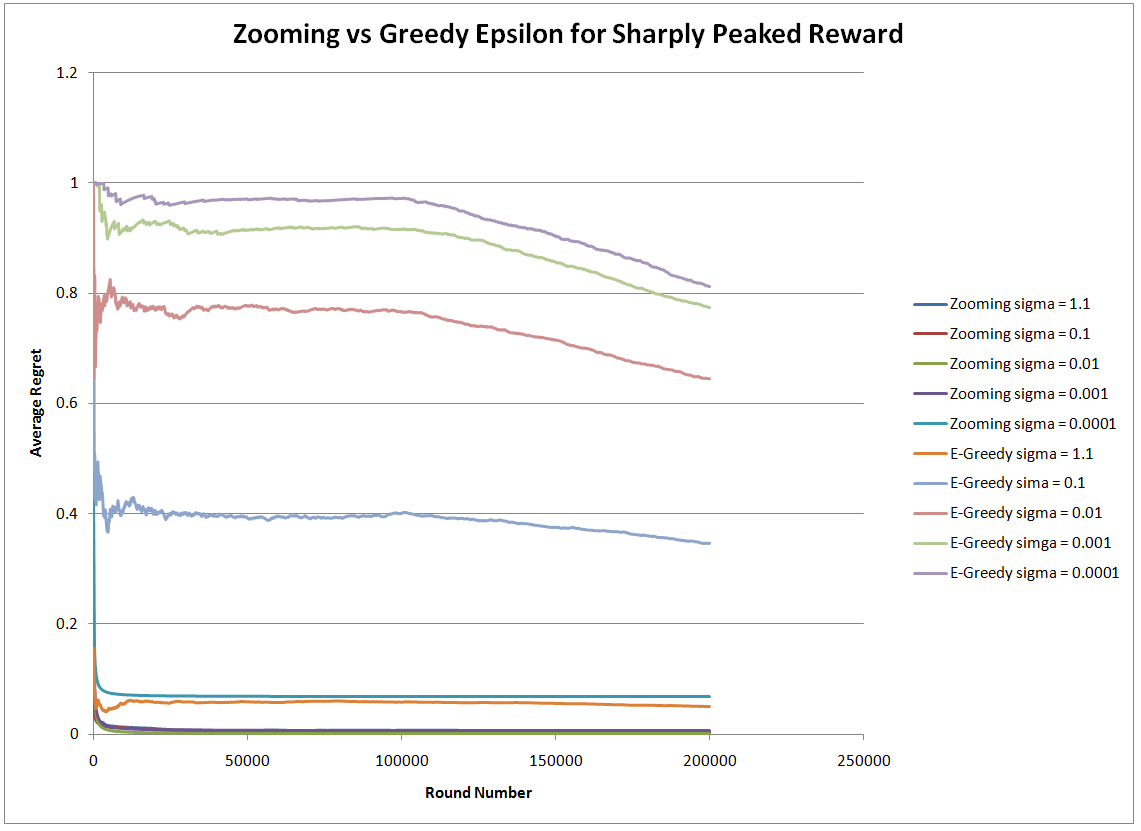
\includegraphics[width=5 in]{figures/ZoomingEpsilonBump.png}
     \caption{The Zooming Algorithm will also eventually home in on the area of max reward, while discretization can simply miss it.}
     \label{fig:zoomebump}
  \end{center}
\end{figure}

\begin{figure}[!ht]
  \begin{center}
    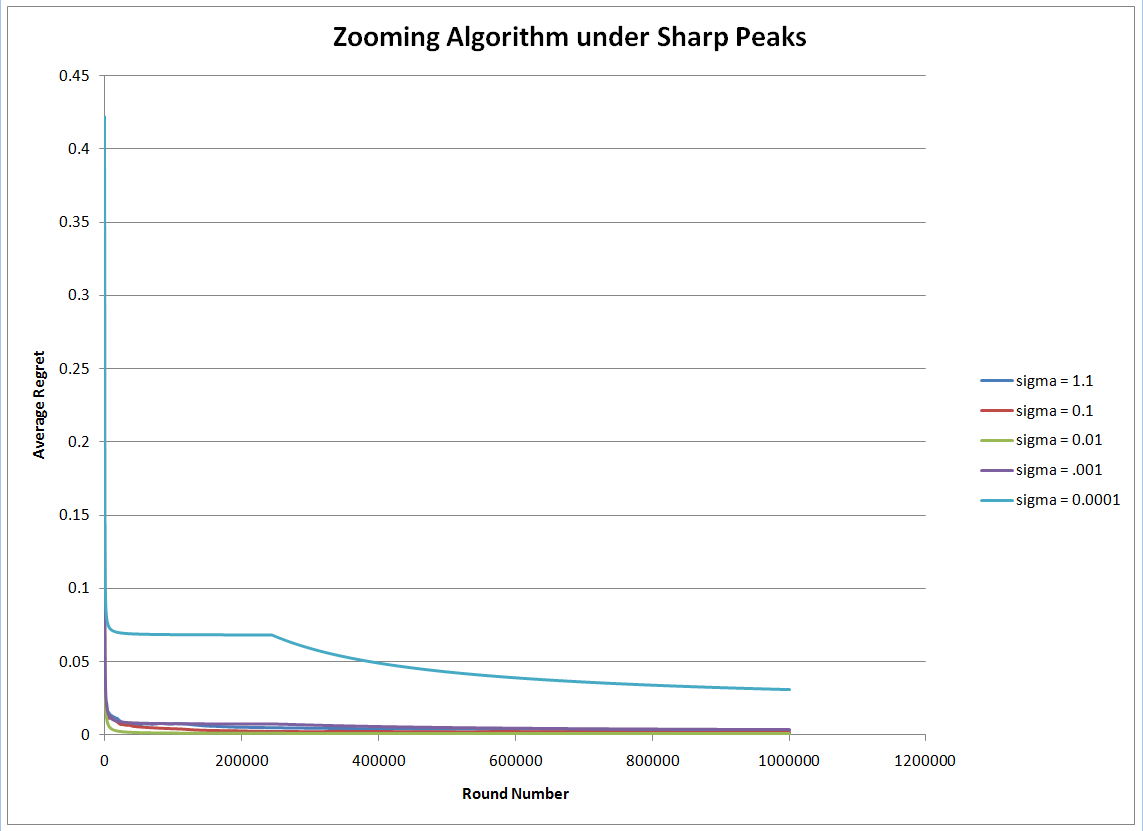
\includegraphics[width=5 in]{figures/ZoomingBump.png}
     \caption{The zooming algorithm takes much longer to find the maximum for very narrow regions, as the radius of coverage decreases }
     \label{fig:zoombump2}
  \end{center}
\end{figure}



These figures show that while discretization algorithms may converge faster, they lack
the resolution in their coverage to detect narrowly peaked maxima, while the algorithms
that progressively refine their coverage will eventually detect them.